\documentclass[]{report}
\usepackage{graphicx}
\graphicspath{ {resources/images/} }


% Title Page
\title{Utilising peer to peer networking for data transfer over the browser}
\author{Dominic Rathbone}


\begin{document}
\maketitle
\tableofcontents
\


\chapter*{Interim Report}
	\section{Project Scope}
		\subsection*{Aims and Objectives}
			The ultimate objective of my project is to investigate the possibility of data transfer over web browsers (in particular audio and video streaming) without the need for a centralised client-server architecture, instead opting for a peer to peer architecture. In order to do so, I will need to research peer to peer networking as well technologies that will allow for it's development in the browser such as WebRTC. In order to test and demonstrate this objective, It will materialize in the form of a web application that people can use to both transfer and stream files (if in a suitable format).
		\subsection*{Stakeholders}
			The stakeholders involved in my project will be myself and the supervisor of my project, Stelios Kapetanakis.
		\subsection*{Methods of Communication}
			Stelios and I have set up a regular meeting once a week on friday at 4pm to review progress and answer any questions. On top of this, we communicate regularly via email and I have set up a private git repository on github to keep my project in which I will give Stelios access to.
		\subsection*{Quality Analysis}
			Success will be measured by the performance of the web application's ability to transfer data. This will be achieved by application metrics recording how fast/reliably files are streamed and transferred under differing amounts of load. Load will be simulated using a load testing tool to mock client connections to the web application.
		
	\section{Specification}
			The first intermediate deliverable will be the signalling server written in Java. This will handle the exchange of client meta data in order to establish the connection between two peers using the web application. I plan to overlap the development of this with the development of my second deliverable, the web application as although they are separate products, manually testing the signalling server will be a lot easier with a partially developed application to test it with.
			
			The second deliverable will be the client side web application the user interacts with in order to select a file as well as handling sending the meta data to the signalling server and managing the peer to peer data transfer and media streaming. In terms of risk, I think this deliverable will be the largest in my project as it is the end product and it relies on WebRTC which is a relatively immature technology. As it is relatively new and it is the only technology at the moment enabling browsers to communicate peer to peer, it has not been tried and tested. This means there is more potential for problems such as security flaws to exist. Security is a concern with peer to peer networking as issues could allow for unwanted access to your private information. Whilst it would be hard to mitigate risks like this from my point of view, I think allowing users of the application to enable authentication on the page where the connection lies would give them a level of access control that could avoid unwanted access.
			
			The third deliverable will be the final report containing documentation and analysis using the metrics	from my application, comparing how it and technologies behind it perform in comparison to others, focusing in particular on how peer to peer over the browser (webRTC) compares to other methods of data transfer and media streaming.
			
	\section{Methodology}
		As a way of tracking the progression of my project, I plan to use Kanban methodology.This is used within software development as a way of incrementally producing applications through iterative development. Whilst, it is similar to scrum, it doesn't have the stricter framework surrounding it which requires a product owner and scrum master. It also avoids overloading developers with restrictive time-boxed sprints. This methodology is relatively simple and based around a backlog of tasks which developers pull from in a limited amount, normally 1 or 2 tasks at a time which will are then pushed through the development work flow. In my case, the work flow will be relatively simple:
			\begin{enumerate}
				\item Development iteration per task
				\begin{itemize}
					\item Coding
					\item Code Review: Code will be reviewed by self-evaluation, static code analysis and reviews from other peers and StackExchange.
					\item Manual Testing: If applicable, black box testing will be used to evaluate the code from a user's perspective.
				\end{itemize}
				\item Stakeholder Approval/User Acceptance Testing: Once all the tasks producing a complete working feature have been completed, it will be tested. 
			\end{enumerate}
		During the coding period of the work flow, I will use a test driven development (TDD) process in which tests are written first and then code is wrote to make the test work. However, I will be fairly lenient with this, only using this process on parts of the code that require stringent testing as writing unnecessary tests will take up development time. 
		\begin{center}
			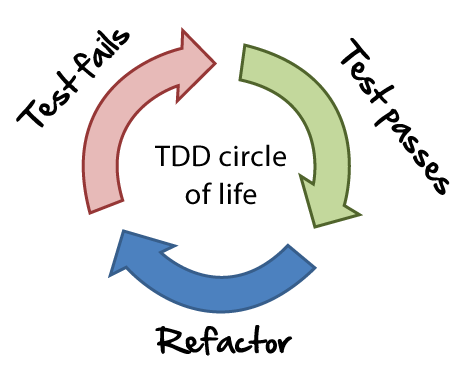
\includegraphics[scale=0.5]{tdd-circle-of-life.png}
		\end{center}

	\section{Literature Review}
		\subsection*{Peer to peer networking}
		The entire idea behind my application is based on a one-to-one peer to peer connection between two browsers. Whilst the connection is formed by WebRTC, it does only this, leaving the application to deal with connecting multiple peers together in a “many-to-many” structure resembling a peer to peer network.
		A peer to peer network 


\end{document}          
